\section{Partner Controller}

VEX Robotics once sold a "partner controller" that allowed a secondary controller to control the robot. However, as of 2021, they are discontinued. 

\begin{figure}[h]
    \centering
    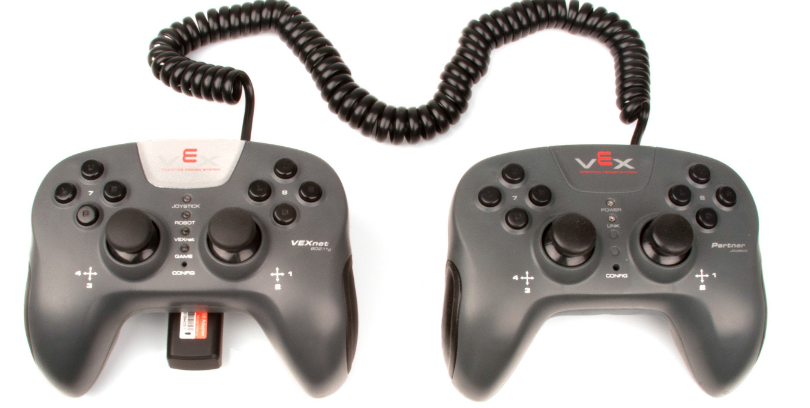
\includegraphics[width=\textwidth,height=10cm,keepaspectratio=true]{PartnerController/PartnerExample}
    \caption{
        A discontinued partner controller (right) being connected to a regular VEXnet controller (left).
    }
\end{figure}

Turns out, the special wire needed to connect VEXnet controllers together is a regular old 4-conductor phone cable \cite{PartnerCite2}. Even better, the regular VEXnet controller has had a firmware update that allows them to be used as a partner controller, meaning you only need to connect two regular controllers together \cite{PartnerCite1}.


\begin{figure}[h]
    \centering
    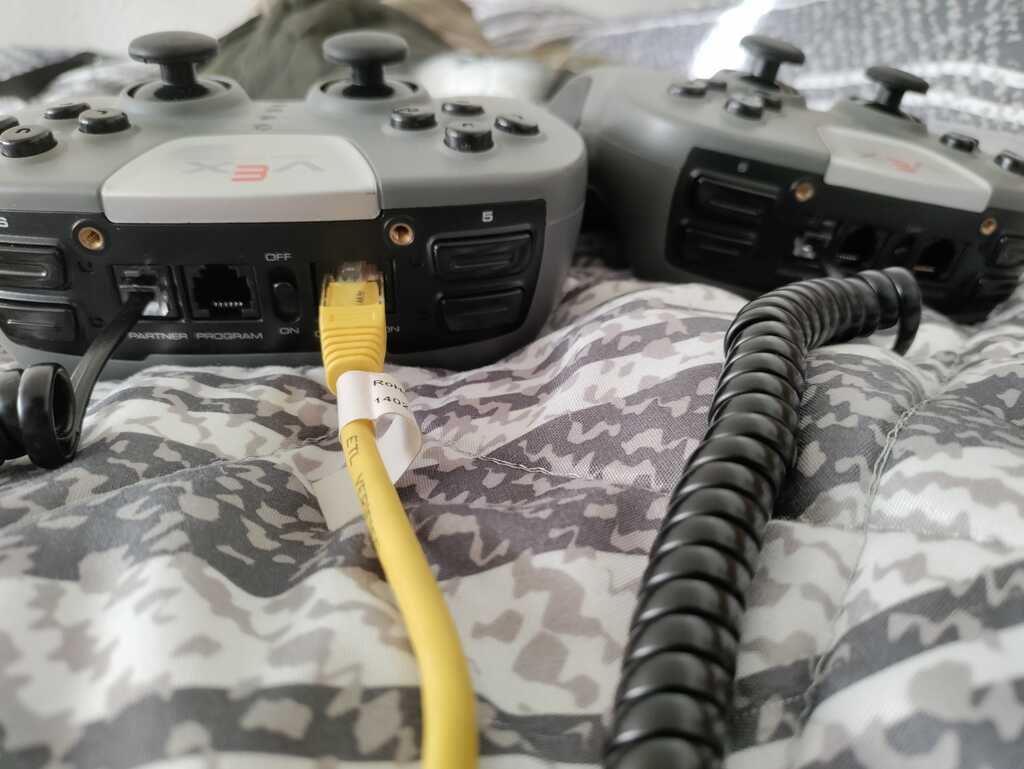
\includegraphics[width=\textwidth,height=7cm,keepaspectratio=true]{PartnerController/Partner1}
    \caption{
        Picture of an ethernet port and telephone port on the VEXnet controller. The telephone cable is used to connect a partner controller, and the ethernet port is used to switch between autonomous and competition mode using a VEX competition switch \cite{VEXCompSwitch}. (You can also make a competition switch yourself \cite{VEXDIYCompSwitch}) The unused port in the middle is a proprietary port used for wireless programming via a VEX programming kit \cite{VEXProgrammingKit}.
    }
\end{figure}


\begin{figure}[h]
    \centering
    \includegraphics[width=\textwidth,height=7cm,keepaspectratio=true]{PartnerController/Partner2}
    \caption{
        Picture of a secondary controller being used to control the robot via a telephone cable connecting both controllers together.
    }
\end{figure}

Along the way, I discovered other ports on the VEXnet controllers; An ethernet cable can be plugged into the controller when using the competition switch, which is important to know if you want to make your own \cite{VEXCompSwitch}. The other port is the programming port that comes with the programming kit for the Cortex for wireless programming, which sadly cannot be built from scratch.
